Much of machine learning is about minimizing a \term{cost function} (also called an \term{objective function} in the optimization community), which is a scalar function of several variables that typically measures how poorly our model fits the data we have.

\subsection{Extrema}
Optimization is about finding \term{extrema}, which depending on the application could be minima or maxima.
When defining extrema, it is also necessary to consider the set of inputs over which we're optimizing.
This set $\calX \subseteq \R^d$ is called the \term{feasible set}.
If $\calX$ is the entire domain of the function being optimized (as it often will be for our purposes), we say that the problem is \term{unconstrained}.
Otherwise the problem is \term{constrained} and may be much harder to solve, depending on the nature of the feasible set.

Suppose $f : \R^d \to \R$.
A point $\x$ is said to be a \term{local minimum} (resp. \term{local maximum}) of $f$ in $\calX$ if $f(\x) \leq f(\y)$ (resp. $f(\x) \geq f(\y)$) for all $\y$ in some neighborhood $\calN \subseteq \calX$ that contains $\x$.
Furthermore, if $f(\x) \leq f(\y)$ for all $\y \in \calX$, then $\x$ is a \term{global minimum} of $f$ in $\calX$ (similarly for global maximum).
If the phrase ``in $\calX$'' is unclear from context, assume we are optimizing over the whole domain of the function.

The qualifier \term{strict} (as in e.g. a strict local minimum) means that the inequality sign in the definition is actually a $>$ or $<$, with equality not allowed.
This indicates that the extremum is unique.

Observe that maximizing a function $f$ is equivalent to minimizing $-f$, so optimization problems are typically phrased in terms of minimization without loss of generality.
This convention (which we follow here) eliminates the need to discuss minimization and maximization separately.

\subsection{Gradients}
The single most important concept from calculus in the context of machine learning is the \term{gradient}.
Gradients generalize derivatives to scalar functions of several variables.
The gradient of $f : \R^d \to \R$ at $\x \in \R^d$, denoted $\nabla f(\x)$, is given by
\[\nabla f(\x) = \matlit{{\pdv{f}{x_1}}(\x) \\ \vdots \\ {\pdv{f}{x_n}}(\x)}\]
Gradients have the following very important property: $\nabla f(\x)$ points in the direction of \term{steepest ascent} from $\x$:
%\begin{center}
%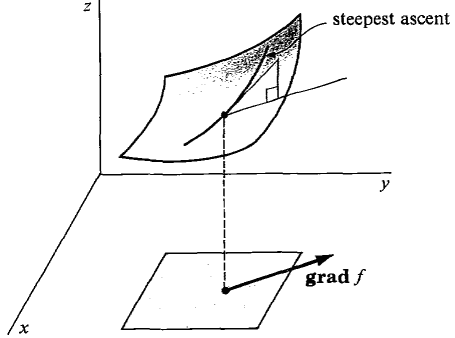
\includegraphics[width=0.9\linewidth]{gradient}
%\end{center}
Similarly, $-\nabla f(\x)$ points in the direction of \term{steepest descent} from $\x$.
We will use this fact frequently when iteratively minimizing a function via \term{gradient descent}.

\subsection{The Jacobian}
The \term{Jacobian} of $f : \R^m \to \R^n$ is a matrix of first-order partial derivatives:
\[\mat{J}_f(\x) = \matlit{
	{\pdv{f_1}{x_1}}(\x) & \hdots & {\pdv{f_1}{x_n}}(\x) \\
	\vdots & \ddots & \vdots \\
	{\pdv{f_m}{x_1}}(\x) & \hdots & {\pdv{f_m}{x_n}}(\x)
}\]
i.e.
\[[\mat{J}_f(\x)]_{ij} = {\pdv{f_i}{x_j}}(\x)\]

\subsection{The Hessian}
The \term{Hessian} matrix of $f : \R^d \to \R$ at $\x \in \R^d$ is a matrix of second-order partial derivatives:
\[\nabla^2 f(\x) = \matlit{
	{\pdv[2]{f}{x_1}}(\x) & \hdots & {\pdv{f}{x_1}{x_n}}(\x) \\
	\vdots & \ddots & \vdots \\
	{\pdv{f}{x_n}{x_1}}(\x) & \hdots & {\pdv[2]{f}{x_n}}(\x)
}\]
i.e.
\[[\nabla^2 f(\x)]_{ij} = {\pdv{f}{x_i}{x_j}}(\x)\]
Recall that if the partial derivatives are continuous, the order of differentiation can be interchanged (Clairaut's theorem), so the Hessian matrix will be symmetric.
This will typically be the case for differentiable functions that we work with.

The Hessian is used in some optimization algorithms such as Newton's method.
It is expensive to calculate but can drastically reduce the number of iterations needed to converge to a local minimum by providing information about the curvature of $f$.

\subsection{Taylor's theorem}
Taylor's theorem has natural generalizations to functions of more than one variable.
One version states
\[f(\x + \y) = f(\x) + \nabla f(\x + \alpha\y)\tran\y\]
for some $\alpha \in (0,1)$.
Furthermore, if $f$ is twice-differentiable, we have
\[f(\x + \y) = f(\x) + \nabla f(\x)\tran\y + \frac{1}{2}\y\tran\nabla^2f(\x+\alpha\y)\y\]
for some $\alpha \in (0,1)$.

This theorem is used in proofs about necessary and sufficient conditions for local optima.
We don't reproduce the proofs here, but the interested reader can consult \cite{numopt}.

Here is an example of such a useful fact: if $f$ is differentiable, then for any extremum $\x$, $\nabla f(\x) = \vec{0}$.
Note that the converse does not hold in general, that is, $\nabla f(\x) = \vec{0}$ does not necessarily imply that $\x$ is an extremum.
(It could be a \term{saddle point} of $f$.)

\subsection{Matrix calculus}
Since a lot of optimization reduces to finding points where the gradient vanishes, it is useful to have differentiation rules for matrix and vector expressions.
We give some common rules here.
Probably the two most important for our purposes are
\begin{align*}
\nabla_\x &(\vec{a}\tran\x) = \vec{a} \\
\nabla_\x &(\x\tran\A\x) = (\A + \A\tran)\x
\end{align*}
Note that this second rule is defined only if $\A$ is square.
Furthermore, if $\A$ is symmetric, we can simplify the result to $2\A\x$.

\subsubsection{The chain rule}
Most functions that we wish to optimize are not completely arbitrary functions, but rather are composed of simpler functions which we know how to handle.
The chain rule gives us a way to calculate derivatives for a composite function in terms of the derivatives of the simpler functions that make it up.

The chain rule from single-variable calculus should be familiar:
\[(f \circ g)'(x) = f'(g(x))g'(x)\]
where $\circ$ denotes function composition.
We can generalize this to the multivariate case.
\begin{proposition}
Suppose $f : \R^m \to \R$ and $g : \R^n \to \R^m$. Then $f \circ g : \R^n \to \R$ and
\[\nabla (f \circ g)(\x) = \mat{J}_g(\x)\tran \nabla f(g(\x))\]
\end{proposition}
\begin{proof}
Observe that each $x_i$ potentially affects every output element of $g$, so we must sum the effects across all of these elements.
The derivative of $f \circ g$ with respect to $x_i$ is given by
\[{\pdv{(f \circ g)}{x_i}}(\x) = \sum_{j=1}^m {\pdv{(f \circ g)}{g_j}\pdv{g_j}{x_i}}(\x) = \nabla f(g(\x))\tran {\pdv{g}{x_i}}(\x)\]
where
\[{\pdv{g}{x_i}}(\x) = \matlit{
{\pdv{g_1}{x_i}}(\x) \\
\vdots \\
{\pdv{g_m}{x_i}}(\x)
}\]
Stacking these partial derivatives and recalling the definitions of the Jacobian matrix and matrix multiplication, we obtain the desired result.
\end{proof}

\subsection{Convexity}
\term{Convexity} is a term that pertains to both sets and functions.
There is a whole branch of mathematics called \term{convex analysis} devoted to studying convexity of sets and functions, but we will just focus on the bits relevant to optimization, particularly convexity as it pertains to functions.

For functions, there are different degrees of convexity, and how convex a function is tells us a lot about its minima: do they exist, are they unique, how quickly can we find them using optimization algorithms, etc.
In this section, we present basic results regarding convexity, strict convexity, and strong convexity.

\subsubsection{Convex sets}
\begin{figure}
  \centering
  \begin{subfigure}[b]{0.45\linewidth}
    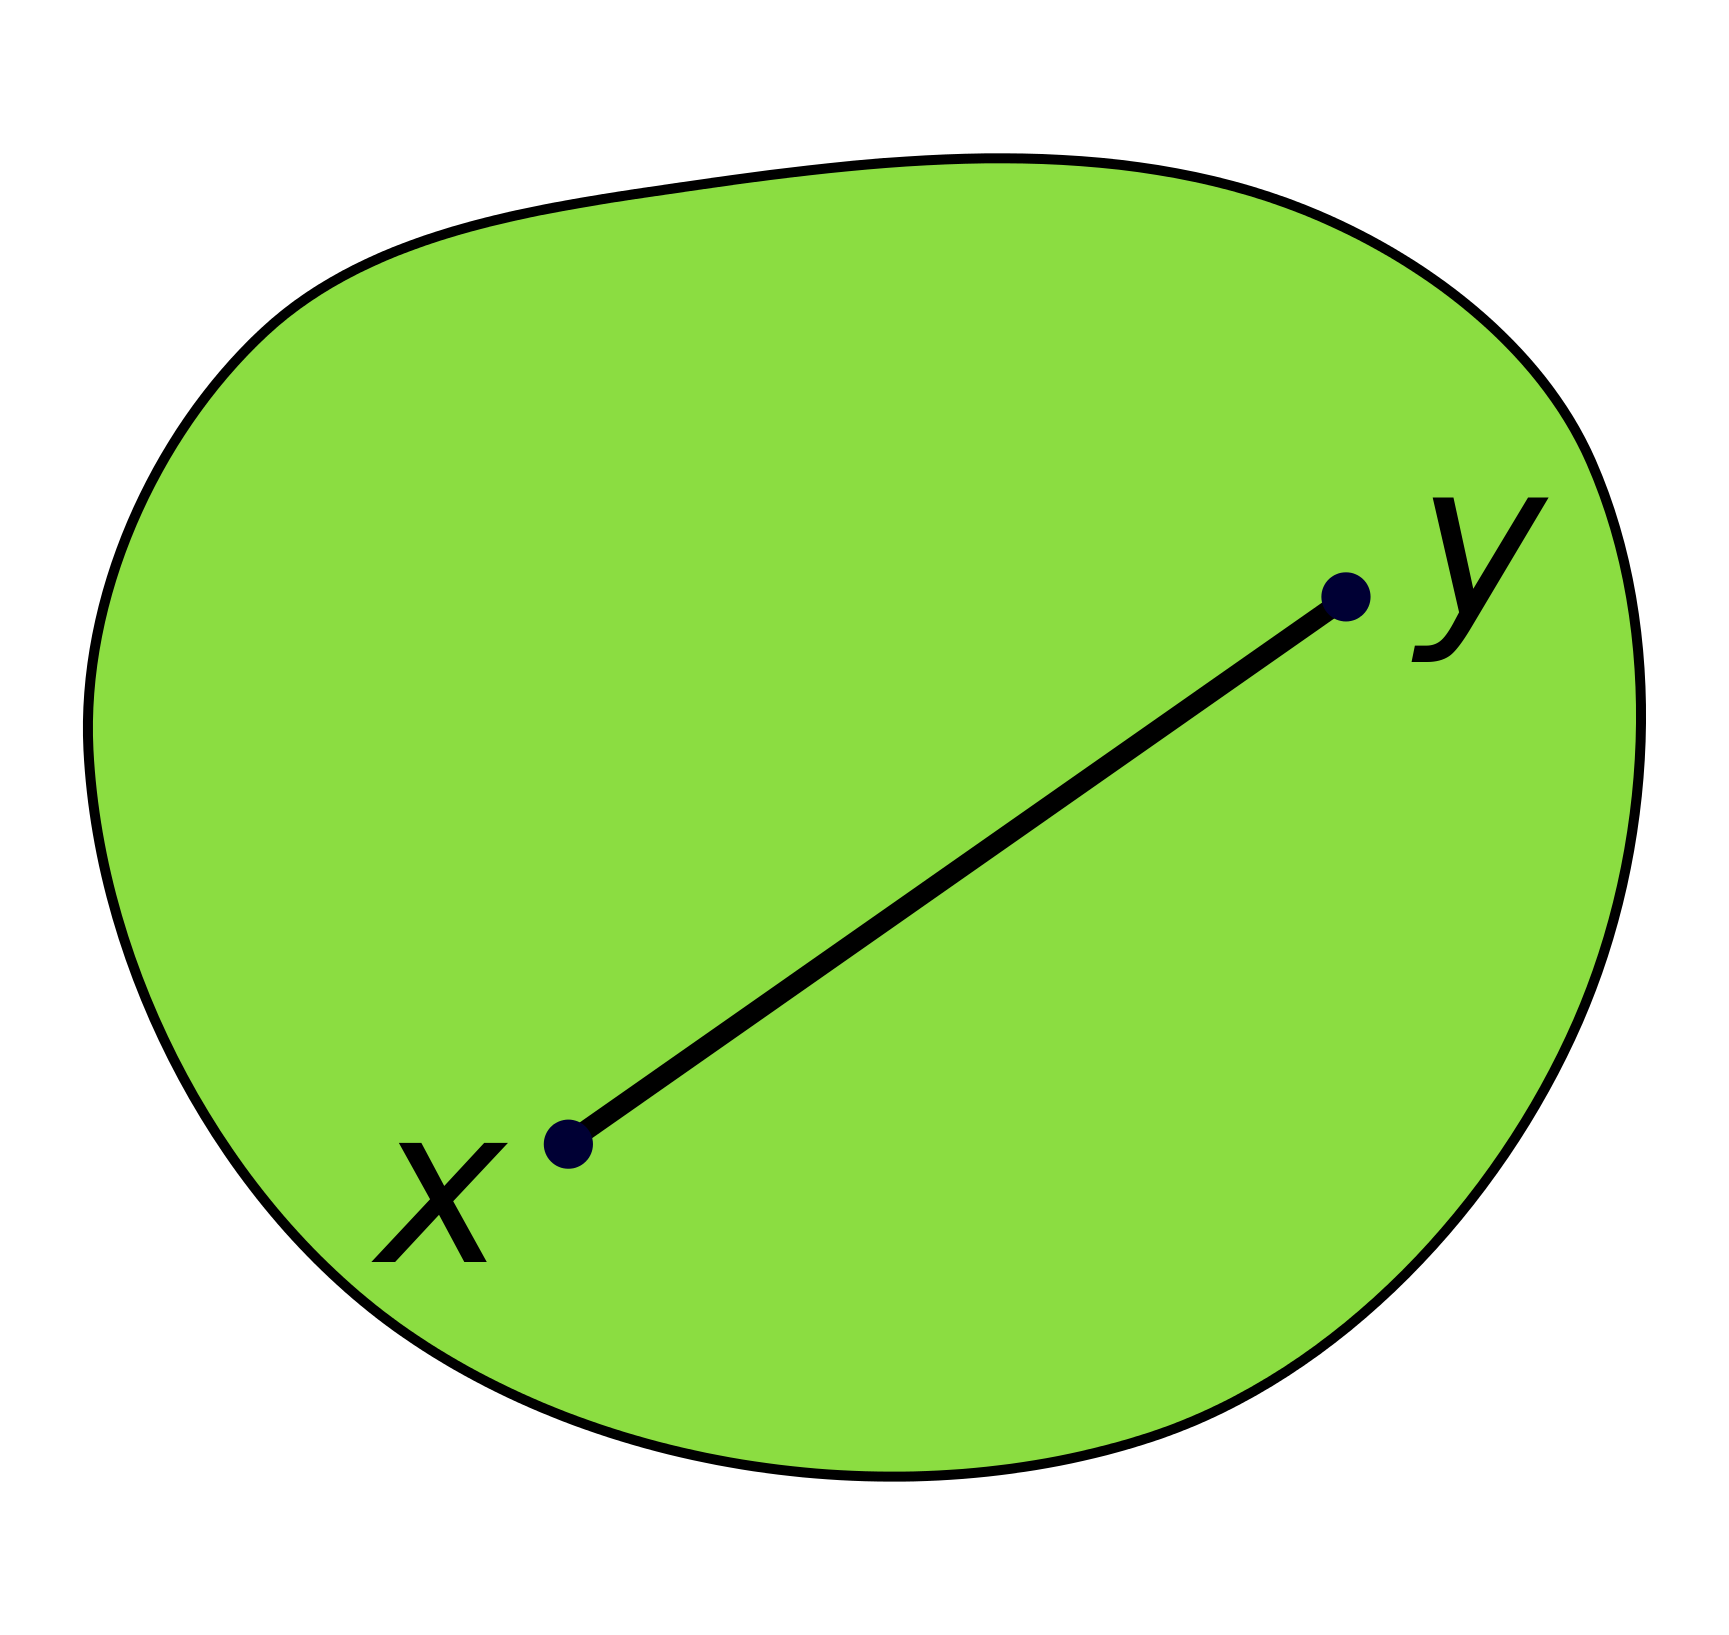
\includegraphics[width=\linewidth]{convex-set}
    \caption{A convex set}
  \end{subfigure}
  \begin{subfigure}[b]{0.45\linewidth}
    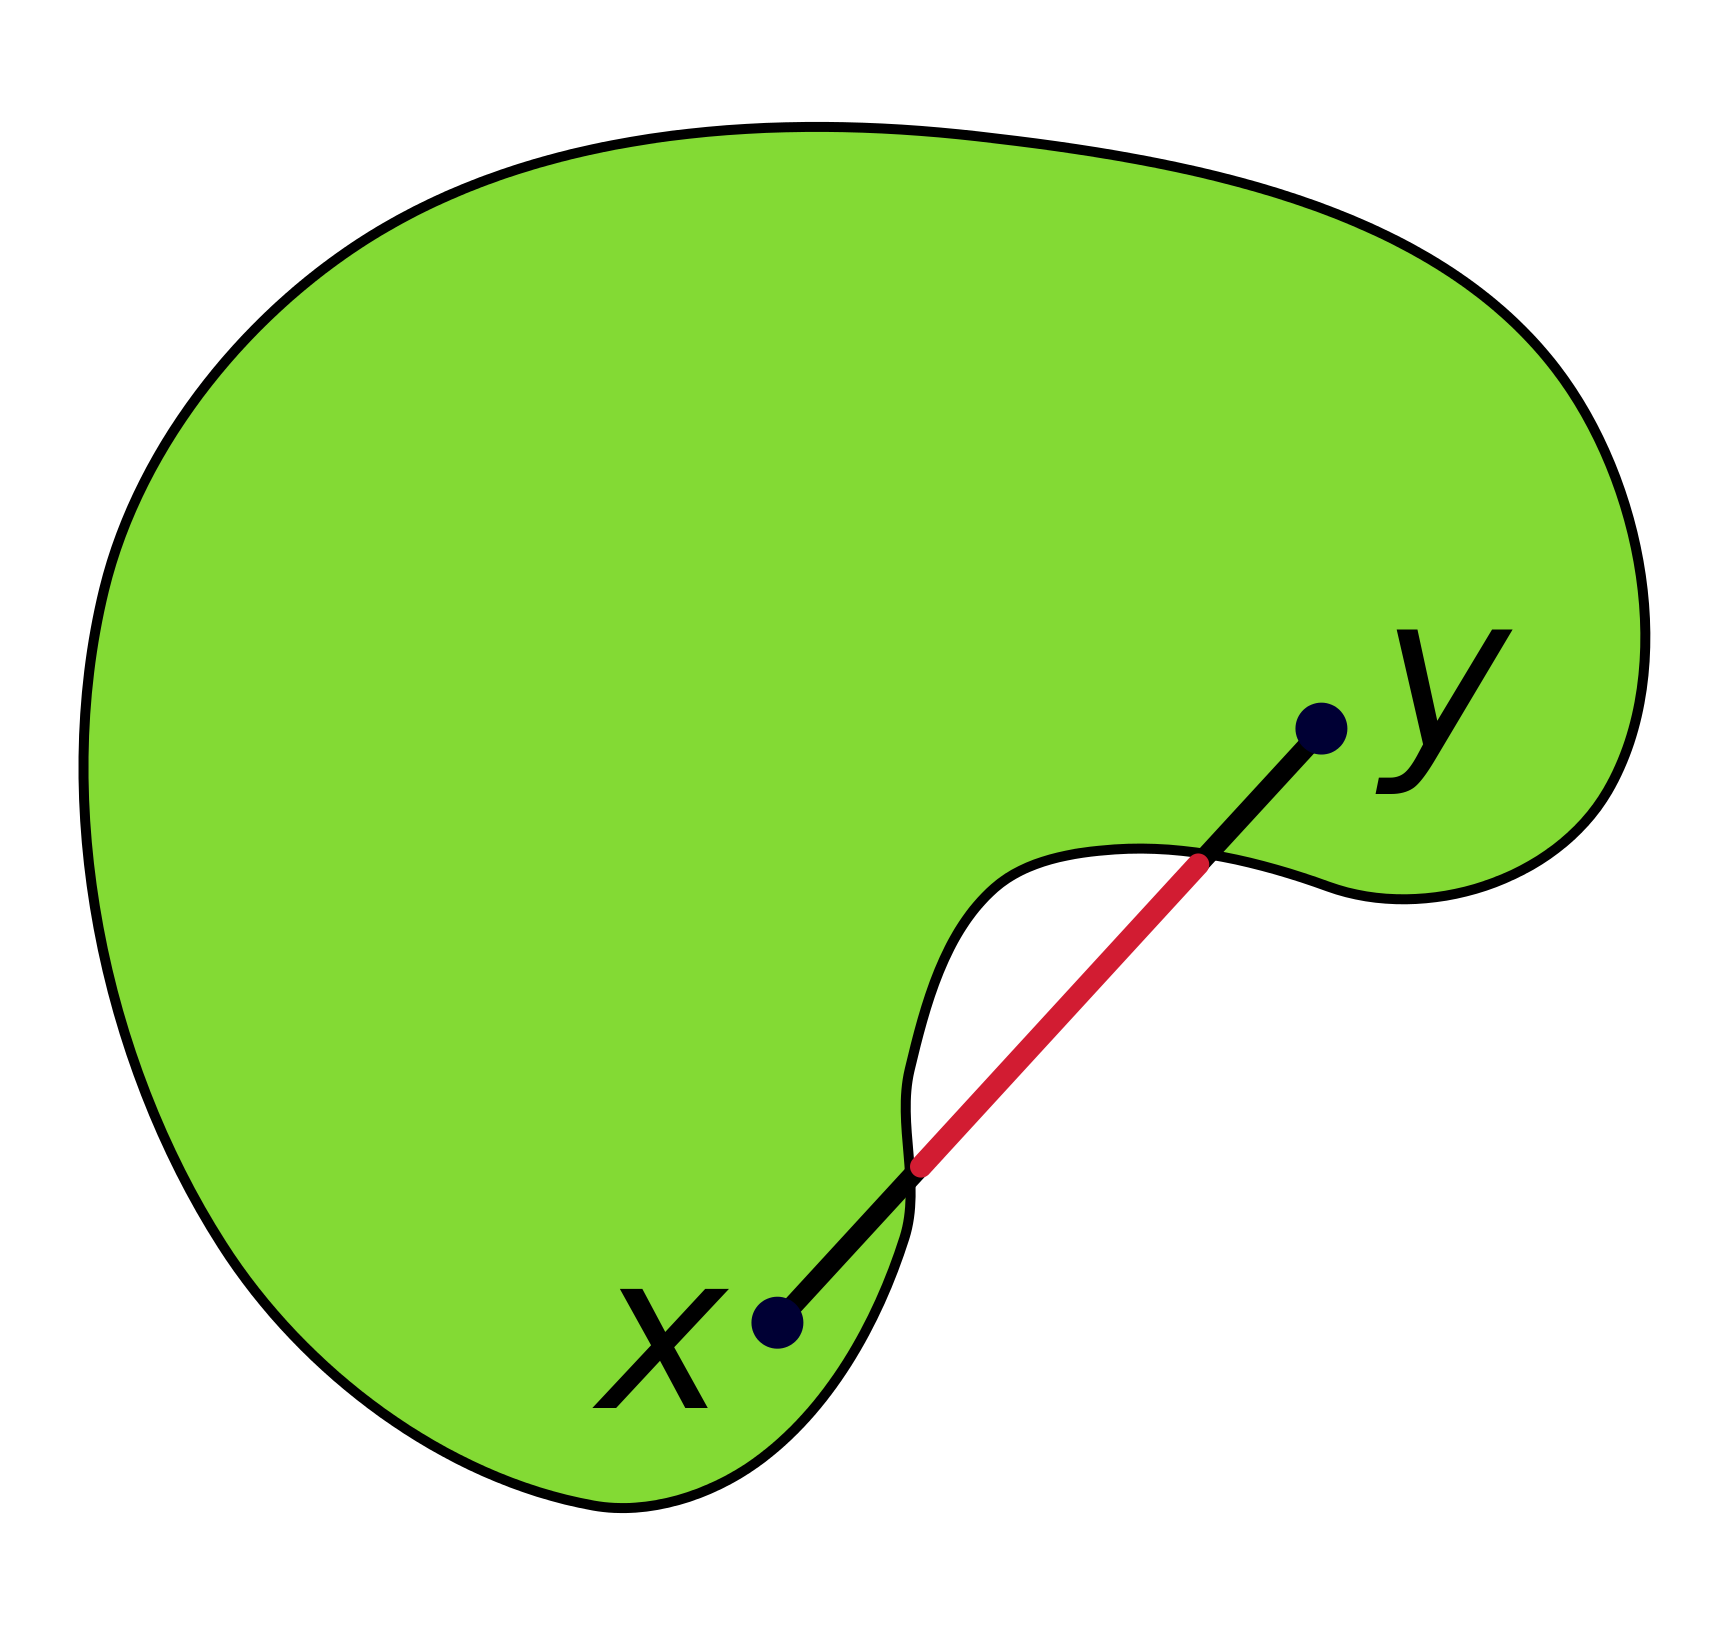
\includegraphics[width=\linewidth]{nonconvex-set}
    \caption{A non-convex set}
  \end{subfigure}
  \caption{What convex sets look like}
  \label{fig:convexset}
\end{figure}

A set $\calC \subseteq \R^d$ is \term{convex} if
\[t\x + (1-t)\y \in \calC\]
for all $\vec{x}, \vec{y} \in \calC$ and all $t \in [0,1]$.

Geometrically, this means that all the points on the line segment between any two points in $\calC$ are also in $\calC$.
See Figure \ref{fig:convexset} for a visual.

Why do we care whether or not a set is convex?
We will see later that the nature of minima can depend greatly on whether or not the feasible set is convex.
Undesirable pathological results can occur when we allow the feasible set to be arbitrary, so for proofs we will need to assume that it is convex.
Fortunately, we often want to minimize over all of $\R^d$, which is easily seen to be a convex set.

\subsubsection{Basics of convex functions}
In the remainder of this section, assume $f : \R^d \to \R$ unless otherwise noted. We'll start with the definitions and then give some results.

A function $f$ is \term{convex} if
\[f(t\vec{x} + (1-t)\vec{y}) \leq t f(\vec{x}) + (1-t)f(\vec{y})\]
for all $\vec{x}, \vec{y} \in \dom f$ and all $t \in [0,1]$.

If the inequality holds strictly (i.e. $<$ rather than $\leq$) for all $t \in (0,1)$ and $\x \neq \y$, then we say that $f$ is \term{strictly convex}.

A function $f$ is \term{strongly convex with parameter $m$} (or \term{$m$-strongly convex}) if the function
\[\x \mapsto f(\x) - \frac{m}{2}\|\x\|_2^2\]
is convex.

These conditions are given in increasing order of strength; strong convexity implies strict convexity which implies convexity.

%\begin{proposition}
%If $f$ is strictly convex, then $f$ is convex.
%\end{proposition}
%\begin{proof}
%Suppose $\x, \y \in \dom f$ and $t \in [0,1]$. We break it down by cases:
%\begin{enumerate}
%\item $\x \neq \y$ and $t \in (0,1)$: the convexity condition is a clear consequence of the strict convexity condition.
%\item $\x = \y$ and $t \in [0,1]$: we have
%\[f(t\x + (1-t)\y) = f(t\x + (1-t)\x) = f(\x) = f(\x) + t f(\x) - t f(\y) = t f(\x) + (1-t)f(\y)\]
%so the condition holds.
%\item $t = 0$: then
%\[f(t\x + (1-t)\y) = f(\y) = t f(\x) + (1-t)f(\y)\]
%\item $t = 1$: similar to the $t = 0$ case.
%\end{enumerate}
%Hence $f$ is convex.
%\end{proof}
%
%\begin{proposition}
%If $f$ is $m$-strongly convex, then $f$ is strictly convex.
%\end{proposition}
%\begin{proof}
%To-do.
%\end{proof}

\begin{figure}
  \centering
  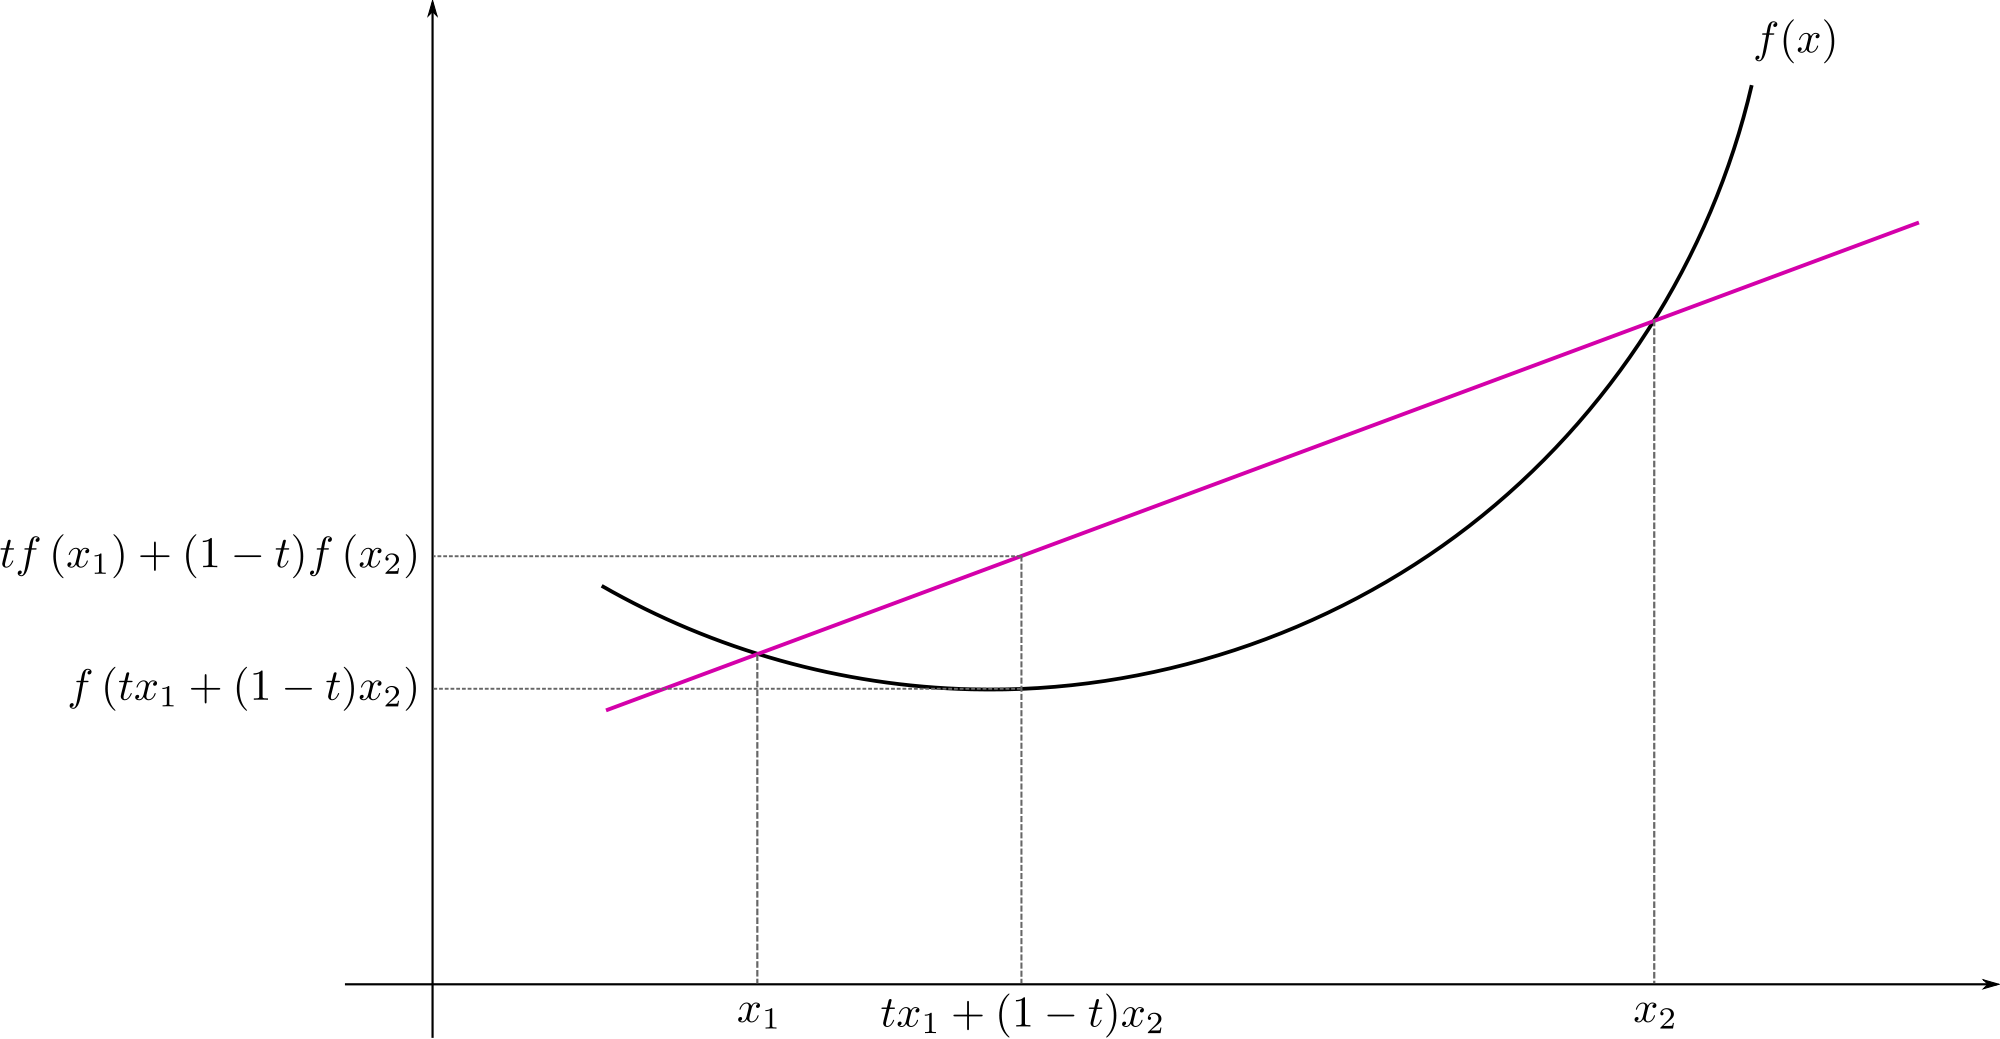
\includegraphics[width=\linewidth]{convex-function}
  \caption{What convex functions look like}
  \label{fig:convexfunction}
\end{figure}

Geometrically, convexity means that the line segment between two points on the graph of $f$ lies on or above the graph itself.
See Figure \ref{fig:convexfunction} for a visual.

Strict convexity means that the graph of $f$ lies strictly above the line segment, except at the segment endpoints.
(So actually the function in the figure appears to be strictly convex.)

\subsubsection{Consequences of convexity}
Why do we care if a function is (strictly/strongly) convex?

Basically, our various notions of convexity have implications about the nature of minima.
It should not be surprising that the stronger conditions tell us more about the minima.

\begin{proposition}
Let $\calX$ be a convex set.
If $f$ is convex, then any local minimum of $f$ in $\calX$ is also a global minimum.
\end{proposition}
\begin{proof}
Suppose $f$ is convex, and let $\x^*$ be a local minimum of $f$ in $\calX$.
Then for some neighborhood $\calN \subseteq \calX$ about $\x^*$,
\[f(\x) \geq f(\x^*) \tab \forall \x \in \calN\]
Suppose towards a contradiction that there exists $\xye \in \calX$ such that $f(\xye) < f(\x^*)$.
Consider the line segment $\x(t) = t\x^* + (1-t)\xye, ~ t \in [0,1]$, noting that $\x(t) \in \calX$ by the convexity of $\calX$.
Then by the convexity of $f$,
\[f(\x(t)) \leq tf(\x^*) + (1-t)f(\xye) < tf(\x^*) + (1-t)f(\x^*) = f(\x^*)\]
for all $t \in (0,1)$.

We can pick $t$ to be sufficiently close to $1$ that $\x(t) \in \calN$; then $f(\x(t)) \geq f(\x^*)$ by the definition of $\calN$, but $f(\x(t)) < f(\x^*)$ by the above inequality, a contradiction.

It follows that $f(\x^*) \leq f(\x)$ for all $\x \in \calX$, so $\x^*$ is a global minimum of $f$ in $\calX$.
\end{proof}

\begin{proposition}
Let $\calX$ be a convex set.
If $f$ is strictly convex, then there exists at most one local minimum of $f$ in $\calX$.
Consequently, if it exists it is the unique global minimum of $f$ in $\calX$.
\end{proposition}
\begin{proof}
The second sentence follows from the first, so all we must show is that if a local minimum exists in $\calX$ then it is unique.

Suppose $\x^*$ is a local minimum of $f$ in $\calX$, and suppose towards a contradiction that there exists a local minimum $\xye \in \calX$ such that $\xye \neq \x^*$.

Since $f$ is strictly convex, it is convex, so $\x^*$ and $\xye$ are both global minima of $f$ in $\calX$ by the previous result.
Hence $f(\x^*) = f(\xye)$.
Consider the line segment $\x(t) = t\x^* + (1-t)\xye, ~ t \in [0,1]$, which again must lie entirely in $\calX$.
By the strict convexity of $f$,
\[f(\x(t)) < tf(\x^*) + (1-t)f(\xye) = tf(\x^*) + (1-t)f(\x^*) = f(\x^*)\]
for all $t \in (0,1)$.
But this contradicts the fact that $\x^*$ is a global minimum.
Therefore if $\xye$ is a local minimum of $f$ in $\calX$, then $\xye = \x^*$, so $\x^*$ is the unique minimum in $\calX$.
\end{proof}

It is worthwhile to examine how the feasible set affects the optimization problem.
We will see why the assumption that $\calX$ is convex is needed in the results above.

Consider the function $f(x) = x^2$, which is a strictly convex function.
The unique global minimum of this function in $\R$ is $x = 0$.
But let's see what happens when we change the feasible set $\calX$.
\begin{enumerate}[(i)]
\item $\calX = \{1\}$: This set is actually convex, so we still have a unique global minimum.
But it is not the same as the unconstrained minimum!

\item $\calX = \R \setminus \{0\}$: This set is non-convex, and we can see that $f$ has no minima in $\calX$.
For any point $x \in \calX$, one can find another point $y \in \calX$ such that $f(y) < f(x)$.

\item $\calX = (-\infty,-1] \cup [0,\infty)$: This set is non-convex, and we can see that there is a local minimum ($x = -1$) which is distinct from the global minimum ($x = 0$).

\item $\calX = (-\infty,-1] \cup [1,\infty)$: This set is non-convex, and we can see that there are two global minima ($x = \pm 1$).
\end{enumerate}

\subsubsection{Showing that a function is convex}
Hopefully the previous section has convinced the reader that convexity is an important property.
Next we turn to the issue of showing that a function is (strictly/strongly) convex.
It is of course possible (in principle) to directly show that the condition in the definition holds, but this is usually not the easiest way.

\begin{proposition}
Norms are convex.
\end{proposition}
\begin{proof}
Let $\|\cdot\|$ be a norm on $\R^d$. Then for all $\x, \y \in \R^d$ and $t \in [0,1]$,
\[\|t\x + (1-t)\y\| \leq \|t\x\| + \|(1-t)\y\| = |t|\|\x\| + |1-t|\|\y\| = t\|\x\| + (1-t)\|\y\|\]
where we have used respectively the triangle inequality, the homogeneity of norms, and the fact that $t$ and $1-t$ are nonnegative.
Hence $\|\cdot\|$ is convex.
\end{proof}

\begin{proposition}
Suppose $f$ is differentiable. Then $f$ is convex if and only if
\[f(\y) \geq f(\x) + \angle{\nabla f(\x), \y - \x}\]
for all $\x, \y \in \dom f$.
\end{proposition}
\begin{proof}
To-do.
\end{proof}

\begin{proposition}
Suppose $f$ is twice differentiable.
Then
\begin{enumerate}[(i)]
\item $f$ is convex if and only if $\nabla^2 f(\x) \succeq 0$ for all $\x \in \dom f$.
\item If $\nabla^2 f(\x) \succ 0$ for all $\x \in \dom f$, then $f$ is strictly convex.
\item $f$ is $m$-strongly convex if and only if $\nabla^2 f(\x) \succeq mI$ for all $\x \in \dom f$.
\end{enumerate}
\end{proposition}
\begin{proof}
Omitted.
\end{proof}

\begin{proposition}
If $f$ is convex and $\alpha \geq 0$, then $\alpha f$ is convex.
\end{proposition}
\begin{proof}
Suppose $f$ is convex and $\alpha \geq 0$. Then for all $\x, \y \in \dom(\alpha f) = \dom f$,
\begin{align*}
(\alpha f)(t\x + (1-t)\y) &= \alpha f(t\x + (1-t)\y) \\
&\leq \alpha\left(tf(\x) + (1-t)f(\y)\right) \\
&= t(\alpha f(\x)) + (1-t)(\alpha f(\y)) \\
&= t(\alpha f)(\x) + (1-t)(\alpha f)(\y)
\end{align*}
so $\alpha f$ is convex.
\end{proof}

\begin{proposition}
If $f$ and $g$ are convex, then $f+g$ is convex.
Furthermore, if $g$ is strictly convex, then $f+g$ is strictly convex, and if $g$ is $m$-strongly convex, then $f+g$ is $m$-strongly convex.
\end{proposition}
\begin{proof}
Suppose $f$ and $g$ are convex. Then for all $\x, \y \in \dom (f+g) = \dom f \cap \dom g$,
\begin{align*}
(f+g)(t\x + (1-t)\y) &= f(t\x + (1-t)\y) + g(t\x + (1-t)\y) \\
&\leq tf(\x) + (1-t)f(\y) + g(t\x + (1-t)\y) & \text{convexity of $f$} \\
&\leq tf(\x) + (1-t)f(\y) + tg(\x) + (1-t)g(\y) & \text{convexity of $g$} \\
&= t(f(\x) + g(\x)) + (1-t)(f(\y) + g(\y)) \\
&= t(f+g)(\x) + (1-t)(f+g)(\y)
\end{align*}
so $f + g$ is convex.

If $g$ is strictly convex, the second inequality above holds strictly for $\x \neq \y$ and $t \in (0,1)$, so $f+g$ is strictly convex.

If $g$ is $m$-strongly convex, then the function $h(\x) \equiv g(\x) - \frac{m}{2}\|\x\|_2^2$ is convex, so $f+h$ is convex.
But
\[(f+h)(\x) \equiv f(\x) + h(\x) \equiv f(\x) + g(\x) - \frac{m}{2}\|\x\|_2^2 \equiv (f+g)(\x) - \frac{m}{2}\|\x\|_2^2\]
so $f+g$ is $m$-strongly convex.
\end{proof}

\begin{proposition}
If $f_1, \dots, f_n$ are convex and $\alpha_1, \dots, \alpha_n \geq 0$, then
\[\sum_{i=1}^n \alpha_i f_i\]
is convex.
\end{proposition}
\begin{proof}
Follows from the previous two propositions by induction.
\end{proof}

\begin{proposition}
If $f$ is convex, then $g(\vec{x}) \equiv f(A\x + \vec{b})$ is convex for any appropriately-sized $A$ and $\b$.
\end{proposition}
\begin{proof}
Suppose $f$ is convex and $g$ is defined like so. Then for all $\x, \y \in \dom g$,
\begin{align*}
g(t\x + (1-t)\y) &= f(A(t\x + (1-t)\y) + \b) \\
&= f(tA\x + (1-t)A\y + \b) \\
&= f(tA\x + (1-t)A\y + t\b + (1-t)\b) \\
&= f(t(A\x + \b) + (1-t)(A\y + \b)) \\
&\leq tf(A\x + \b) + (1-t)f(A\y + \b) & \text{convexity of $f$} \\
&= tg(\x) + (1-t)g(\y)
\end{align*}
Thus $g$ is convex.
\end{proof}

\begin{proposition}
If $f$ and $g$ are convex, then $h(\vec{x}) \equiv \max\{f(\vec{x}), g(\vec{x})\}$ is convex.
\end{proposition}
\begin{proof}
Suppose $f$ and $g$ are convex and $h$ is defined like so. Then for all $\x, \y \in \dom h$,
\begin{align*}
h(t\x + (1-t)\y) &= \max\{f(t\x + (1-t)\y), g(t\x + (1-t)\y)\} \\
&\leq \max\{tf(\x) + (1-t)f(\y), tg(\x) + (1-t)g(\y)\} \\
&\leq \max\{tf(\x), tg(\x)\} + \max\{(1-t)f(\y), (1-t)g(\y)\} \\
&= t\max\{f(\x), g(\x)\} + (1-t)\max\{f(\y), g(\y)\} \\
&= th(\x) + (1-t)h(\y)
\end{align*}
Note that in the first inequality we have used convexity of $f$ and $g$ plus the fact that $a \leq c, b \leq d$ implies $\max\{a,b\} \leq \max\{c,d\}$.
In the second inequality we have used the fact that $\max\{a+b, c+d\} \leq \max\{a,c\} + \max\{b,d\}$.

Thus $h$ is convex.
\end{proof}

\subsubsection{Examples}
A good way to gain intuition about the distinction between convex, strictly convex, and strongly convex functions is to consider examples where the stronger property fails to hold.

Functions that are convex but not strictly convex:
\begin{enumerate}[(i)]
\item $f(\x) = \w\tran\x + \alpha$ for any $\w \in \R^d, \alpha \in \R$.
Such a function is called an \term{affine function}, and it is both convex and concave.
(In fact, a function is affine if and only if it is both convex and concave.)
Note that linear functions and constant functions are special cases of affine functions.
\item $f(\x) = \|\x\|_1$
\end{enumerate}

Functions that are strictly but not strongly convex:
\begin{enumerate}[(i)]
\item $f(x) = x^4$.
This example is interesting because it is strictly convex but you cannot show this fact via a second-order argument (since $f''(0) = 0$).
\item $f(x) = \exp(x)$.
This example is interesting because it's bounded below but has no local minimum.
\item $f(x) = -\log x$.
This example is interesting because it's strictly convex but not bounded below.
\end{enumerate}

Functions that are strongly convex:
\begin{enumerate}[(i)]
\item $f(\x) = \|\x\|_2^2$
\end{enumerate}

